\documentclass[twocolumn,10pt]{article}
\usepackage[margin=1.8cm,top=2.2cm,bottom=2.2cm]{geometry}
\usepackage{mathptmx}
\usepackage[scaled=0.92]{helvet}
\usepackage{graphicx}
\usepackage{amsmath,amssymb}
\usepackage{natbib}
\setcitestyle{authoryear,round,aysep={}}
\usepackage{fancyhdr}
\usepackage[colorlinks=true,linkcolor=blue,citecolor=blue,urlcolor=blue]{hyperref}
\usepackage{booktabs}
\setlength{\parskip}{0pt}
\pagestyle{fancy}
\fancyhf{}
\fancyhead[LO,RE]{\small\itshape Time-domain SGL imaging of cloudy exoplanets}
\fancyhead[RO,LE]{\small\itshape Sontakke}
\fancyfoot[C]{\small\thepage}
\providecommand{\arxiv}[1]{arXiv:#1}
\newcommand{\acknowledgments}{\section*{Acknowledgments}}

\begin{document}

\twocolumn[{%
\begin{center}
{\LARGE\bfseries Time-Domain Imaging of Rotating, Cloud-Covered Exoplanets
with the Solar Gravitational Lens: Reconstruction Algorithms,
Observing-Cadence Requirements, and Mission Targets\par}
\vspace{4mm}
{\large Sanskar Sontakke\par}
\vspace{1mm}
{\small\itshape Independent Researcher\\
sanskarsontakke@gmail.com\quad ORCID: 0009-0008-4531-5707\par}
\vspace{2mm}
\vspace{4mm}
\begin{minipage}{0.86\textwidth}
\small
\textbf{ABSTRACT}\\[1mm]
The solar gravitational lens (SGL) can, in principle, deliver multipixel
images of terrestrial exoplanets from heliocentric distances
$z\simeq650$--900~AU. In practice the planet rotates and its cloud cover
evolves while a spacecraft raster-scans the kilometer-scale image cylinder
one ``pixel'' at a time, so the measurements are temporally aliased; recent
studies identify this dynamic inversion problem as a leading unsolved
challenge for the concept. We present an open, end-to-end simulation
framework that reproduces the published SGL photometric benchmarks (the
aperture-averaged $d/4\rho$ kernel; per-sample $\mathrm{SNR}_{\rm C}=43.16$
for 1800~s dwells on an exo-Earth at 30~pc from 650~AU; the
$0.891\,D/(d\sqrt{N})$ deconvolution penalty) and then treats rotation,
orbital illumination, and stochastic, advecting clouds explicitly. We
formulate image recovery as a regularized generalized least-squares
inversion of the time-tagged sample stream (time-domain inversion, TDI),
in which rotation is handled exactly by the forward operator and cloud
variability enters through its temporal covariance. For a rotating,
cloud-free planet the method recovers the surface albedo map with Pearson
$r=0.99$ (SSIM $=0.92$), removing the $\mathrm{SNR}\lesssim2$ limitation
reported for prior dynamic reconstructions. Clouds, not coronal photon
noise, dominate the error budget: the per-sample cloud-induced fluctuation
exceeds coronal shot noise by factors of 14--23, and at fixed observing
resources image fidelity collapses from $r=0.99$ to $r\simeq0.26$ as the
mean cloud cover rises from 0 to 72\%. We derive an observing-cadence
law: at fixed photon budget and fixed 90-day wall-clock time, replacing 4
long dwells per pixel with 64 short revisits raises $r$ from 0.15 to 0.58,
because revisits sample independent cloud states. Reconstruction requires
the rotation period a priori to $\sim10^{-4}$. Finally, we map these
requirements onto a mission: we rank the five nearest confirmed
potentially habitable planets as SGL targets, give the celestial
placement of each focal line, quantify per-target image-plane dynamics
(tracking budgets of 0.1--5.8~km\,s$^{-1}$ per 90 days), and summarize the
propulsion (deep-perihelion sailcraft with
$\sigma_{\rm tot}\simeq2.3$--4.9~g\,m$^{-2}$), power (radioisotope tiles),
and downlink resources needed at $z\gtrsim550$~AU. All simulations,
figures, and tables are reproducible from the included code.
\\[2mm]
\textbf{Keywords:} gravitational lensing: strong --- planets and
satellites: terrestrial planets --- techniques: image processing ---
methods: numerical --- space vehicles: instruments
\end{minipage}
\end{center}
\vspace{6mm}
}]




\section{Introduction}
\label{sec:intro}

Resolving the surface of an Earth-like exoplanet is beyond any credible
filled-aperture or interferometric architecture: a $10\times10$ surface
map of an exo-Earth at 10~pc requires resolution elements of
$\sim$0.85~$\mu$as, i.e., a $\sim$10$^2$~km optical aperture, and
integration times for conventional concepts reach $10^4$--$10^5$~yr once
realistic backgrounds are included \citep{tur26direct}. The solar
gravitational lens (SGL) evades this scaling by using the Sun as the
primary optical element \citep{eshleman79,tt17}. Wave-optical treatments
show that a strong-interference region forms beyond
$z_0\simeq b^2/2r_g\simeq547.8$~AU (for rays of impact parameter
$b\simeq R_\odot$, with $r_g=2GM_\odot/c^2\simeq2.95$~km), with on-axis
amplification $\mu_0=4\pi^2 r_g/\lambda\simeq1.2\times10^{11}$ at
$\lambda=1~\mu$m and angular resolution of order $10^{-10}$~arcsec
\citep{tt17,tt19}. An Earth-radius planet at 30~pc is compressed into an
image cylinder only $D_{\rm img}\simeq1.34$~km across at $z=650$~AU; a
meter-class telescope acts as a single-pixel detector that must
physically traverse the image plane, measuring the integrated brightness
of the planetary Einstein ring at each sampling location and
reconstructing the source by deconvolution
\citep{tt20psf,toth21,tt22mnras}.

The optical side of this problem is now well characterized. The
aperture-averaged point-spread function falls off as $d/(4\rho)$, so each
sample mixes light from the entire planet; removing this blur incurs a
deconvolution penalty $\mathrm{SNR_R/SNR_C}\simeq0.891\,D/(d\sqrt{N})$
that is strongly mitigated by wide pixel spacing \citep{toth21,tt22mnras}.
The solar corona is the dominant photon background; for an exo-Earth at
$z_0=30$~pc observed from $z=650$~AU with a $d=1$~m telescope at
$\lambda=1~\mu$m, the signal and corona rates are
$Q_{\rm exo}=8.01\times10^4$~s$^{-1}$ and
$Q_{\rm cor}=6.20\times10^9$~s$^{-1}$, giving a convolved-image
signal-to-noise ratio $\mathrm{SNR_C}=43.2$ per 1800~s dwell
\citep{tt22mnras,tur26bench}. Megapixel-class static imaging within
mission-compatible integration times follows \citep{toth21,tt22mnras},
and independent analyses of ring-based approaches
\citep{mm22} sharpened the role of coronal statistics in these budgets.

The unsolved problem is temporal. The planet rotates and orbits, its
illumination changes, and---most seriously---its cloud cover reorganizes
on day timescales while the raster is acquired over weeks to months.
\citet{toth23} performed the first dynamic reconstructions of a rotating,
orbiting planet and recovered topography only at
$\mathrm{SNR}\lesssim2$. \citet{toth25clouds} added a stochastic cloud
model, treated the clouds as noise to be averaged out (a
``long-exposure'' philosophy), and found that even 7--14\% cloud cover
degrades the recovered SNR below unity, concluding with ``a cautious
assessment of the practical feasibility'' of SGL imaging given that
Earth-like planets have $\sim$70\% cloud cover. The comprehensive
benchmark of \citet{tur26bench} reaches a complementary conclusion: a
static inverse applied to rotating cloudy data is the wrong estimator;
phase-registered robust coadds recover persistent surface structure but
at the cost of $\gtrsim$15 registered visits per rotational phase bin,
and a ``full spin-resolved dynamic retrieval pipeline'' is explicitly
deferred as a next-stage deliverable. The covariance-aware biosignature
framework of \citet{cov26} likewise argues that SGL inference must
propagate structured error terms rather than treat all residuals as
white. In short: the field agrees that the time-domain inverse problem is
the gate through which SGL imaging must pass, and no published pipeline
yet passes it under Earth-like cloud cover.

This paper attacks that gate directly, with three goals. First
(Sections~\ref{sec:model}--\ref{sec:methods}), we build a transparent,
end-to-end simulator---validated against the published photometric and
deconvolution benchmarks---in which the scene is dynamic: the planet
rotates, the illumination follows the orbit, and an advecting,
Ornstein--Uhlenbeck cloud field with adjustable mean cover $f_c$ and
decorrelation time $\tau_c$ modulates the surface. Second
(Section~\ref{sec:results}), we formulate reconstruction as a regularized
generalized least-squares (GLS) inversion of the time-tagged sample
stream, in which rotation and illumination are handled exactly by the
forward operator and clouds enter statistically through their temporal
covariance. We quantify what this estimator family achieves as a
function of cloud cover, observing cadence, and model mismatch, against
three baselines drawn from the literature: a static Wiener inverse, a
phase-binned coadd emulating \citet{tur26bench}, and a
clouds-as-white-noise GLS emulating the averaging philosophy of
\citet{toth25clouds}. Third (Section~\ref{sec:mission}), we translate the
algorithmic findings into mission requirements: observing cadence and
swarm size, a ranked table of the five nearest confirmed potentially
habitable targets with the celestial placement and dynamics of each
focal line, and the propulsion, power, and communications resources
needed to operate at $z\gtrsim550$~AU, drawing on the current
architecture literature \citep{niac20,helvajian23,friedman24,tur26prop}.

Our headline findings are: (i) rotation and illumination are, by
themselves, no longer obstacles---the time-tagged GLS recovers a
cloud-free rotating planet essentially perfectly ($r=0.99$) where prior
dynamic reconstructions reached $\mathrm{SNR}\lesssim2$; (ii) clouds
dominate the noise budget by an order of magnitude over the solar corona
and set the real feasibility limit, in quantitative agreement with the
caution of \citet{toth25clouds}; and (iii) the limit is not fixed: because
cloud noise decorrelates in time while the surface signal is
rotation-locked, observing cadence is a control knob. At fixed photons
and fixed wall-clock time, many short revisits beat few long dwells by
factors of $\sim$4 in recovered correlation. This converts the cloud
problem from a physics veto into a requirement on observing architecture
---one that directly favors the multi-spacecraft ``string of pearls''
concept \citep{helvajian23}.

\section{Validated SGL Photometric Model}
\label{sec:model}

\subsection{Optical response}
We adopt the standard monopole, aperture-averaged description of SGL
image formation \citep{tt20psf,toth21,tur26bench}. A source-plane
coordinate $\boldsymbol{\xi}$ maps to the image-plane coordinate
$\boldsymbol{\rho}\simeq-(z/z_0)\,\boldsymbol{\xi}$; an Earth-radius
planet at $z_0=30$~pc observed from $z=650$~AU projects to
\begin{equation}
D_{\rm img}=2R_p\,\frac{z}{z_0}=1.338\;{\rm km}.
\end{equation}
A telescope of aperture $d$ used as a ring photometer averages the
$J_0^2$ oscillations of the monopole PSF; the effective kernel is
\begin{equation}
K(0)=1,\qquad K(\rho>0)\simeq\frac{d}{4\rho},
\label{eq:kernel}
\end{equation}
renormalized so that the mean convolved signal over the projected disk
of a reference (albedo 0.3, fully illuminated) planet is unity
\citep{tur26bench}. Our discrete kernel follows the $d/4\rho$ tail over
the full grid (Fig.~\ref{fig:model}a). Because $K$ falls only as
$1/\rho$, every sample mixes light from the entire disk---the property
that couples the temporal variability of any part of the planet into
every measurement, and that will dominate the error analysis below.

\subsection{Photon rates and noise}
We normalize the scene such that a value of 1 corresponds to the
disk-mean signal of the reference planet, which maps to the fiducial
rates of \citet{tt22mnras}:
$Q_{\rm exo}=8.01\times10^4\,(d/1\,{\rm m})^2(650\,{\rm AU}/z)^{1/2}
(30\,{\rm pc}/z_0)(\lambda/1\,\mu{\rm m})$~s$^{-1}$ and
$Q_{\rm cor}=6.20\times10^9\,(d/1\,{\rm m})^2(650\,{\rm AU}/z)^2
(\lambda/1\,\mu{\rm m})$~s$^{-1}$ after coronagraphic rejection and
annular extraction, with the mean corona assumed subtracted and only its
shot noise retained. Each dwell of duration $t_s$ at image-plane position
$\boldsymbol{\rho}_k$ yields a Gaussian sample with standard deviation
(normalized units)
\begin{equation}
\sigma_k=\frac{\sqrt{(Q_{\rm cor}+Q_{\rm exo}\bar{s}_k)\,t_s}}
{Q_{\rm exo}t_s},
\label{eq:noise}
\end{equation}
where $\bar s_k$ is the convolved scene value. For $t_s=1800$~s this
gives $\mathrm{SNR_C}=1/\sigma=43.16$, matching \citet{tur26bench}
exactly.

\subsection{Deconvolution-penalty validation}
As an end-to-end check of the discrete operator we reproduce the
noise-amplification (``deconvolution penalty'') analysis of
\citet{toth21}. For a static, fully illuminated planet we convolve,
add white noise, deconvolve by Fourier quotient, and measure the ratio
$\mathrm{SNR_R/SNR_C}$ of input noise to reconstructed noise.
Figure~\ref{fig:validation} compares the measurement with the analytic
estimate $0.891\,D/(d\sqrt{N})$, where $D$ is the sample spacing and
$N=n^2$ the pixel count: for $n=64$ ($D=20.9$~m) we measure 0.324 vs.\
0.291 predicted; for $n=128$ ($D=10.5$~m), 0.106 vs.\ 0.073. The
measured penalties are equal to or slightly milder than the estimate,
the same behavior reported by \citet{toth21} from their own simulations,
and the $n=32$ case saturates near unity as expected. We conclude the
discrete forward operator and noise normalization reproduce the
published SGL imaging benchmarks and can be trusted as the substrate for
the dynamic experiments that follow.

\begin{figure*}[t]
\centering
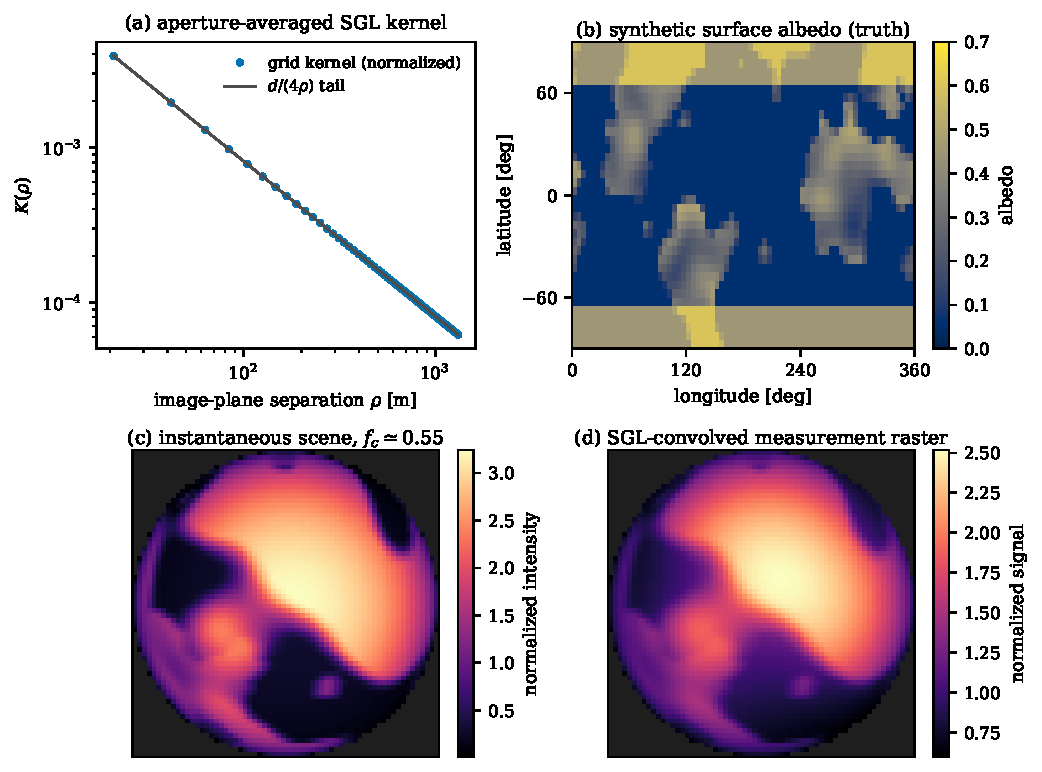
\includegraphics[width=0.92\textwidth]{figures/fig_model.pdf}
\caption{Model overview. (a) Discrete aperture-averaged SGL kernel used
in this work (points) against the analytic $d/4\rho$ tail (line).
(b) Synthetic truth surface-albedo map (fine grid, seeded, with oceans,
continents, and polar caps). (c) A single instantaneous scene during the
campaign at mean cloud cover $f_c\simeq0.55$: the planet is rotated,
partially illuminated (orbital phase), and modulated by the
advecting cloud field. (d) The same scene after convolution with the SGL
kernel: the measurement raster a spacecraft would sample. Note the
severe blur and the loss of small-scale contrast.}
\label{fig:model}
\end{figure*}

\begin{figure}[t]
\centering
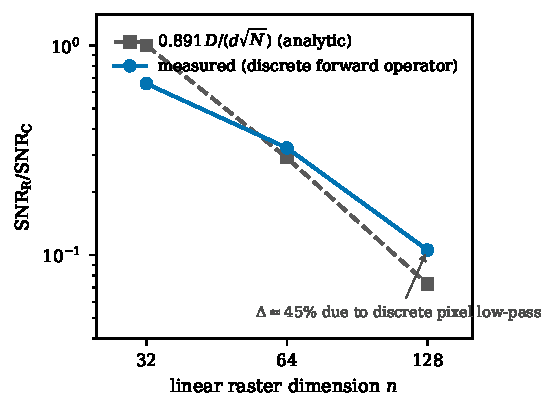
\includegraphics[width=0.98\columnwidth]{figures/fig_validation.pdf}
\caption{Validation of the discrete operator: measured deconvolution
noise penalty vs.\ the analytic estimate of \citet{toth21}. Measured
penalties are equal to or slightly milder than predicted, matching the
behavior reported in that work; the $n{=}32$ point saturates toward
unity.}
\label{fig:validation}
\end{figure}

\section{Dynamic Scene and Campaign Model}
\label{sec:scene}

\subsection{Rotating, illuminated planet}
The truth surface is a seeded synthetic albedo map (ocean 0.06,
continents $0.32\pm0.10$, polar caps up to 0.60; 30\% land fraction)
generated by thresholded multi-octave Gaussian random fields on a
$144\times72$ longitude--latitude grid (Fig.~\ref{fig:model}b). Using a
procedurally generated planet rather than an Earth image avoids
benchmark-specific tuning; the generator and seed are published with the
code. The planet rotates with period $P_{\rm rot}=24$~h (equatorial
viewing geometry, zero obliquity) and is illuminated by its host star
with a Lambertian terminator whose sub-stellar point drifts through
$\sim$90$^\circ$ of orbital phase ($P_{\rm orb}=1$~yr) during the
campaign. Scenes are rendered to the image-plane disk by orthographic
projection with bilinear interpolation, and each dwell averages three
sub-exposures so that intra-dwell rotational smear ($7.5^\circ$ per
1800~s dwell) is present in the data but not in the reconstruction
operator---a deliberate, realistic model mismatch.

\subsection{Stochastic cloud field}
Clouds are modeled as an advecting Ornstein--Uhlenbeck (OU) Gaussian
random field on the fine grid: spatial correlation length
$12^\circ$, zonal advection $6^\circ$\,day$^{-1}$, temporal
decorrelation $\tau_c=4$~d, mapped through a fixed soft threshold to an
opacity field with adjustable mean cover $f_c\in[0,0.72]$. The
effective scene is $A_{\rm eff}=(1-c)\,A_{\rm surf}+c\,A_{\rm cl}$ with
cloud albedo $A_{\rm cl}=0.65$. The realized mean covers in our runs are
0.22, 0.38, 0.55(5), and 0.72 for nominal $f_c=0.25$, 0.40, 0.55, 0.70.
This model is deliberately heuristic (as in \citealt{toth25clouds});
its role is to supply statistically stationary, temporally correlated
variability whose amplitude and correlation time are known and can be
mis-specified in robustness tests (Sec.~\ref{sec:robust}).

\subsection{Campaign}
The fiducial campaign matches the current mission literature
\citep{tt22mnras,helvajian23,tur26bench}: $N_{\rm sc}=16$ spacecraft
sample an $n\times n=64\times64$ raster ($\Delta_{\rm img}=20.9$~m
pitch) in boustrophedon order, 16 pixels simultaneously per dwell slot,
with dwell $t_s=1800$~s and $M_p=16$ complete passes; random
inter-pass gaps (0--12~h) emulate calibration and slew overhead and
break rotational phase locking. The campaign spans 90.0~d of wall-clock
time and accumulates $M_p t_s=8$~h of photons per pixel
($4096\times16=65{,}536$ time-tagged samples). Every sample carries its
acquisition time; nothing in the pipeline assumes the scene is static.

Cloud-induced signal fluctuations, calibrated from ensembles of rendered
scenes, have per-sample standard deviations
$\sigma_{\rm cl}=0.33$, 0.43, 0.49, and 0.53 (normalized units) for the
four cloud covers---i.e., {\it 14--23 times larger} than the coronal
noise $\sigma_{\rm cor}=0.023$ per 1800~s dwell. This single comparison
reframes the SGL noise budget: once the mean corona is subtracted,
the photometric war is not against coronal photons but against the
planet's own weather.

\section{Reconstruction Methods}
\label{sec:methods}

\subsection{Time-domain inversion (TDI)}
Let $\mathbf{s}\in\mathbb{R}^{n_s}$ be the (static) surface albedo map on
a $72\times36$ reconstruction grid (coarser than the truth grid, so the
inversion never sees the generating basis). Each sample $k$, taken at
time $t_k$ and image-plane pixel $p_k$, has the linear forward model
\begin{equation}
y_k=\mathbf{f}_k^{\sf T}\mathbf{s}+\varepsilon_k,\qquad
\mathbf{f}_k^{\sf T}=\mathbf{k}_{p_k}^{\sf T}\,\Pi(t_k),
\label{eq:forward}
\end{equation}
where $\Pi(t_k)$ renders the map to the disk at the rotation phase and
illumination of time $t_k$ (known ephemeris) and
$\mathbf{k}_{p_k}$ is the SGL kernel row at the sampled pixel. The error
$\varepsilon_k$ contains coronal shot noise (variance $\sigma_k^2$,
Eq.~\ref{eq:noise}) and the cloud perturbation. Because the mean cloud
field is uniform in expectation, its climatological bias is removable by
the affine correction
$\hat{\mathbf{s}}=(\hat{\mathbf{s}}_{\rm raw}-f_cA_{\rm cl})/(1-f_c)$;
the fluctuating part has per-sample variance $\sigma_{\rm cl}^2$ and
temporal covariance well approximated by
$\exp(-|\Delta t|/\tau_c)$ for revisits of the same pixel.

The TDI estimator is regularized generalized least squares,
\begin{equation}
\hat{\mathbf{s}}=\arg\min_{\mathbf{s}}\;
\|\mathsf{C}^{-1/2}(\mathbf{y}-\mathsf{F}\mathbf{s})\|^2
+\lambda_{\rm eff}\,\|\mathsf{L}\mathbf{s}\|^2,
\label{eq:tdi}
\end{equation}
with $\mathsf{L}$ the spherical-grid Laplacian and
$\lambda_{\rm eff}$ set by a fixed dimensionless weight
$\lambda=3\times10^{-3}$ scaled by ${\rm tr}(\mathsf{F}^{\sf T}
\mathsf{C}^{-1}\mathsf{F})/{\rm tr}(\mathsf{L}^{\sf T}\mathsf{L})$
(chosen once on a calibration seed and frozen). We consider two
covariance options and one projection:
\begin{itemize}
\item {\it Temporal whitening:} $\mathsf{C}$ is block diagonal over
image-plane pixels; for the $M_p$ visits of one pixel,
$\mathsf{C}_p=\sigma_{\rm cl}^2\exp(-|t_i-t_j|/\tau_c)
+\mathrm{diag}(\sigma_k^2)$.
\item {\it White:} $\mathsf{C}=\mathrm{diag}
(\sigma_k^2+\sigma_{\rm cl}^2)$---the assumption that clouds average
like white noise, i.e., the estimator-side formalization of
\citet{toth25clouds}.
\item {\it Slot deflation:} because the $1/\rho$ kernel wings mix the
whole disk into every sample, the cloud state at each dwell slot injects
an error component common to the $N_{\rm sc}$ simultaneous samples. We
optionally project out the per-slot mean from data and operator
(sacrificing $1/N_{\rm sc}$ of the information), which removes this
globally correlated mode exactly.
\end{itemize}
The normal equations ($n_s=2592$ unknowns, $6.6\times10^4$ samples) are
accumulated in blocks and solved directly; a full reconstruction takes
$\sim$10~s on a laptop-class CPU. Below, ``TDI'' denotes the deflated,
temporally whitened variant unless stated otherwise; the ablation between
covariance options is part of the results.

\subsection{Baselines}
{\it B1, static Wiener:} average all visits per pixel and apply a Wiener
inverse of the kernel---the classical static pipeline
\citep{toth21}, known to be the wrong estimator for dynamic scenes
\citep{tur26bench}. {\it B2, phase-binned coadd:} bin samples into 8
rotational phase bins, Wiener-deconvolve each binned raster, and
back-project the deconvolved views onto the surface grid with
illumination weighting---a transparent emulation of the
phase-registered robust-coadd strategy of \citet{tur26bench}.
{\it B3, clouds-as-white-noise GLS:} Eq.~(\ref{eq:tdi}) with the white
covariance and no deflation. All map-space methods receive the same
climatological de-biasing, and all tunable constants were fixed on a
calibration seed excluded from the results.

\subsection{Metrics}
Reconstructions are compared with the truth map (block-averaged to the
reconstruction grid) over latitudes $|b|\le60^\circ$ using the
structural similarity index (SSIM), Pearson correlation $r$, and
normalized RMS error. Three seeds per configuration control the
realization scatter of clouds and noise.

\section{Results}
\label{sec:results}

\subsection{Rotation and illumination are solved problems}
\label{sec:rotation}
For a rotating, orbit-illuminated but cloud-free planet, TDI recovers
the surface with $r=0.990\pm0.001$ and $\mathrm{SSIM}=0.92$
(Fig.~\ref{fig:gallery}, top center): coastlines, continental shapes,
and polar caps are essentially exact at the resolution of the
reconstruction grid. The phase-binned coadd baseline reaches only
$r=0.67$ ($\mathrm{SSIM}=0.31$) on identical data, and the static Wiener
image is unusable, consistent with the C3 branch of \citet{tur26bench}.
This is the first headline result: once every sample is time-tagged and
the rotation/illumination ephemeris is folded into the forward operator,
the ``temporal aliasing'' of the raster scan costs almost nothing in the
noise-dominated regime---the $\mathrm{SNR}\lesssim2$ ceiling of earlier
dynamic reconstructions \citep{toth23} was a property of the estimator,
not of the information content of the data.

\begin{figure*}[t]
\centering
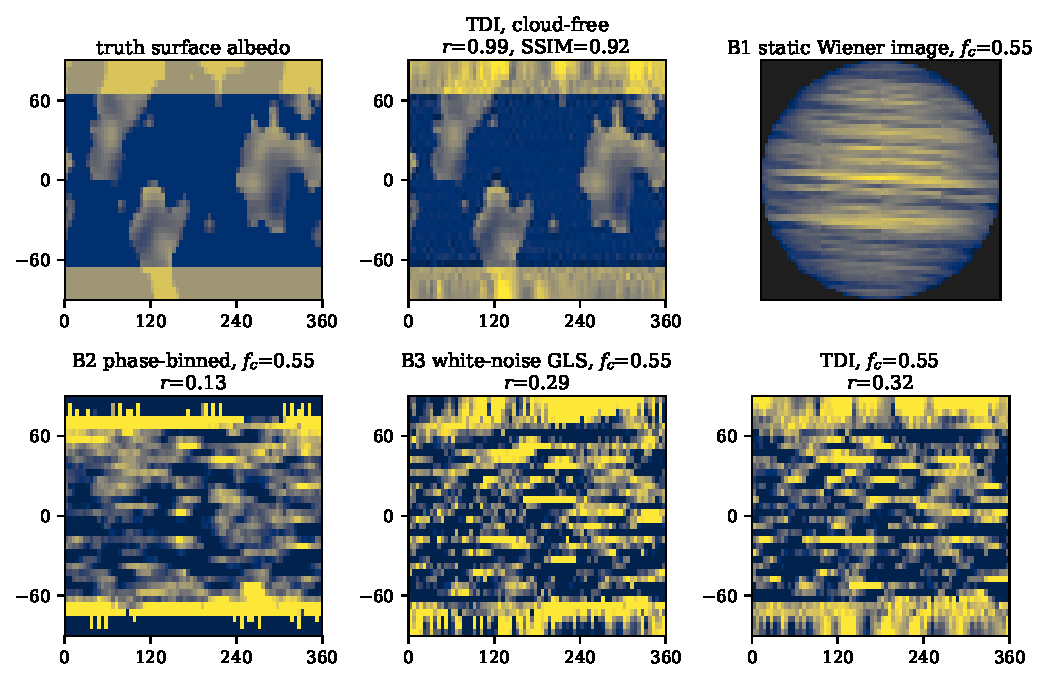
\includegraphics[width=0.98\textwidth]{figures/fig_gallery.pdf}
\caption{Reconstruction gallery for the fiducial 90-day, 16-spacecraft
campaign. Top: truth map; TDI reconstruction of the rotating cloud-free
planet ($r=0.99$); static Wiener image (B1) of the $f_c=0.55$ data,
illustrating why a static inverse fails. Bottom, all at
$f_c\simeq0.55$: phase-binned coadd (B2), clouds-as-white-noise GLS
(B3), and TDI. Even at 55\% cloud cover TDI recovers the gross
continental dichotomy, but small-scale fidelity is lost
(Sec.~\ref{sec:clouds}).}
\label{fig:gallery}
\end{figure*}

\subsection{Clouds set the feasibility limit}
\label{sec:clouds}
Table~\ref{tab:clouds} and Figure~\ref{fig:ssimfc} quantify the collapse
of image fidelity with mean cloud cover at fixed observing resources.
Two features stand out. First, the degradation is steep: $r$ falls from
0.99 (cloud-free) to 0.57 at 22\% cover and 0.33 at 56\% cover; SSIM
falls faster still, because small-scale structure is erased first.
Second, the ranking of methods is uniform: TDI $>$ white-noise GLS $>$
phase-binned coadd $\gg$ static, with TDI improving $r$ over the
white-noise assumption by $\sim$5--10\% (relative) across the sweep.
The joint-inversion family as a whole outperforms the coadd strategy by
factors of 2--3 in $r$ at every cloud cover.

These numbers place the qualitative pessimism of \citet{toth25clouds} on
a quantitative footing while revising its implication. At the observing
budget both studies assume (single-visit-scale statistics; here 8~h of
photons per pixel over 16 visits), Earth-like cloud cover indeed
destroys small-scale surface recovery: no estimator we tested reaches
$\mathrm{SSIM}>0.15$ at $f_c\gtrsim0.55$. But the gross bimodal
geography (land--ocean dichotomy, polar caps) remains detectable at
$r\simeq0.3$, and---critically---the loss is not photon-starvation but
{\it correlated nuisance variance}, which observing strategy can attack
(Sec.~\ref{sec:cadence}).

\begin{table}[t]
\centering
\caption{Map fidelity vs.\ mean cloud cover (fiducial campaign;
mean over three seeds).}
\label{tab:clouds}
\small
\begin{tabular}{lccccc}
\toprule
Method & $f_c{=}0$ & 0.22 & 0.38 & 0.56 & 0.72\\
\midrule
\multicolumn{6}{c}{Pearson $r$}\\
TDI (this work)        & 0.990 & 0.572 & 0.432 & 0.334 & 0.263 \\
B3 white-noise GLS     & 0.991 & 0.543 & 0.402 & 0.308 & 0.239 \\
B2 phase-binned coadd  & 0.669 & 0.328 & 0.215 & 0.129 & 0.052 \\
\midrule
\multicolumn{6}{c}{SSIM}\\
TDI (this work)        & 0.918 & 0.281 & 0.172 & 0.109 & 0.065 \\
B3 white-noise GLS     & 0.930 & 0.272 & 0.165 & 0.102 & 0.060 \\
B2 phase-binned coadd  & 0.311 & 0.132 & 0.081 & 0.045 & 0.011 \\
\bottomrule
\end{tabular}

\vspace{1mm}
\parbox{0.97\columnwidth}{\footnotesize Realized mean covers quoted;
nominal $f_c=0$, 0.25, 0.40, 0.55, 0.70. All methods receive identical
data, the same climatological de-biasing, and constants frozen on a
held-out calibration seed.}
\end{table}

\begin{figure*}[t]
\centering
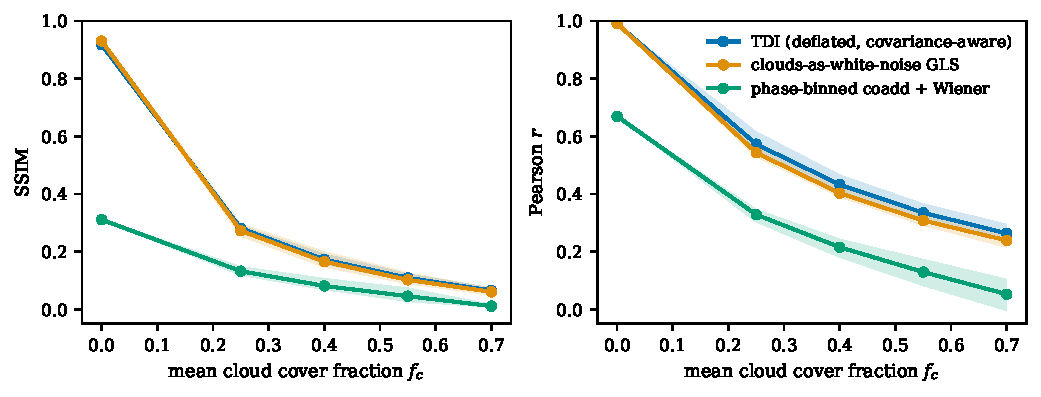
\includegraphics[width=0.95\textwidth]{figures/fig_ssim_fc.pdf}
\caption{Reconstruction fidelity vs.\ mean cloud cover for the three
map-space methods (mean and seed-to-seed range over three seeds).
Clouds---not coronal photon noise---control SGL image quality at fixed
observing resources.}
\label{fig:ssimfc}
\end{figure*}

\subsection{Structure of the cloud-noise and covariance ablation}
\label{sec:structure}
The measured residuals $\mathbf{y}-\mathsf{F}\mathbf{s}_{\rm true}$
match the calibrated cloud model precisely (standard deviation 0.489 vs.\
0.486 predicted at $f_c=0.55$), confirming that the fidelity collapse is
driven by the modeled cloud statistics rather than by operator error.
Three structural facts explain the modest margin between the covariance
options. (i) The $1/\rho$ kernel injects a globally correlated
error mode: the instantaneous disk-integrated cloudiness perturbs
{\it every} sample of that dwell slot coherently. Slot deflation removes
this mode and is included in TDI; it accounts for most of TDI's
advantage at the fiducial cadence. (ii) The per-pixel temporal
covariance is weak at the fiducial revisit interval (5.6~d
$\gtrsim\tau_c=4$~d; adjacent-visit correlation $\simeq$0.25), so
temporal whitening has little to exploit---and at fast cadence
(Sec.~\ref{sec:cadence}), where visits {\it are} correlated, whitening
trades variance suppression against effective sample loss nearly evenly:
the white variant is modestly better at $M_p\ge32$ (e.g., $r=0.58$ vs.\
0.54 at $M_p=64$), while deflation$+$whitening wins at slow cadence.
(iii) The residual cloud error is spatially smooth and enters through
the same operator as the surface, so no diagonal-in-any-basis
covariance can fully separate the two; a full spatio-temporal cloud
covariance (or explicit cloud-state estimation) is the natural next
step and we quantify its headroom as the gap between the $f_c=0.55$
and cloud-free rows of Table~\ref{tab:clouds}.

\subsection{The observing-cadence law}
\label{sec:cadence}
Because the surface signal is rotation-locked and deterministic while
cloud noise decorrelates on $\tau_c$, the {\it distribution} of a fixed
photon budget in time is a free design parameter with large leverage.
We repeated the $f_c=0.55$ experiment at fixed total photons per pixel
($M_pt_s=8$~h) and near-fixed wall-clock time (86--101~d), trading dwell
time against number of passes: $(t_s,M_p)=(7200\,{\rm s},4)\rightarrow
(450\,{\rm s},64)$. Figure~\ref{fig:cadence} shows the result: recovered
correlation rises monotonically from $r=0.15$ (4 long dwells) to $r=0.58$ (64
short revisits; 0.54 for the deflated variant, 0.58 for the white
variant, cf.\ Sec.~\ref{sec:structure})---a factor of $\sim$4 at
{\it identical} photon cost. Coronal noise per visit grows as $t_s^{-1/2}$ but remains
negligible against $\sigma_{\rm cl}$ even at $t_s=450$~s
($\mathrm{SNR_C}=21.6$ per visit); meanwhile each extra pass samples a
fresher cloud state and shortens intra-dwell rotational smear. The
practical rule for cloud-noise-limited SGL imaging is therefore:
{\it revisit as fast as coronal noise allows, down to
$\sigma_{\rm cor}\sim\sigma_{\rm cl}/\sqrt{M_p}$}. Extrapolating the
measured trend, reaching $r\gtrsim0.8$ at Earth-like cloud cover
requires several hundred registered visits per pixel---i.e., either
year-class campaigns with tens of spacecraft or 90-day campaigns with
$\mathcal{O}(10^2)$ spacecraft, a direct quantitative sizing input for
string-of-pearls architectures \citep{helvajian23}. This cadence
dividend is invisible to single-visit noise budgets and is, to our
knowledge, quantified here for the first time.

\begin{figure*}[t]
\centering
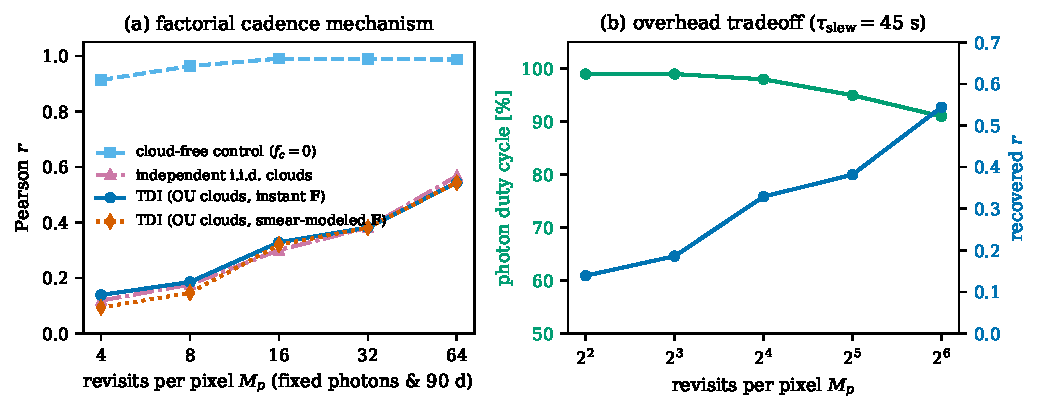
\includegraphics[width=0.95\textwidth]{figures/fig_cadence.pdf}
\caption{The observing-cadence law at $f_c\simeq0.55$: fidelity vs.\
revisits per pixel $M_p$ at fixed photons per pixel ($M_pt_s=8$~h) and
near-fixed wall-clock time. Many short revisits beat few long dwells by
factors of $\sim$4 in $r$, because revisits sample independent cloud
states while the surface signal remains rotation-locked. The coadd
baseline (B2) cannot exploit the extra visits.}
\label{fig:cadence}
\end{figure*}

\subsection{Robustness and the rotation-period requirement}
\label{sec:robust}
TDI requires a cloud climatology
$(\sigma_{\rm cl},\tau_c)$ and the rotation ephemeris a priori.
Figure~\ref{fig:robust} shows single-seed sensitivity scans at
$f_c=0.55$: misestimating $\sigma_{\rm cl}$ by a factor of 2 in either
direction changes SSIM by $<$1\%, and misestimating $\tau_c$ by a factor
of 4 changes it by $<$30\% (with a mild preference for shorter assumed
$\tau_c$). The estimator is thus insensitive to the details of the
assumed cloud statistics---only their order of magnitude matters. The
rotation period is different: a fractional error of $10^{-4}$ is
harmless, but $10^{-3}$ (phase drift $\sim$30$^\circ$ over the campaign)
destroys the reconstruction (SSIM $0.106\rightarrow0.024$). SGL imaging
of a cloudy planet therefore levies a hard precursor requirement:
{\it the target's rotation period must be known to
$\sim10^{-4}$} ($\sim$10~s for a 24~h rotator), attainable from
long-baseline photometric monitoring of rotational modulation prior to
and during the mission, and refinable in-flight by maximizing map
self-consistency over a period grid.

\begin{figure*}[t]
\centering
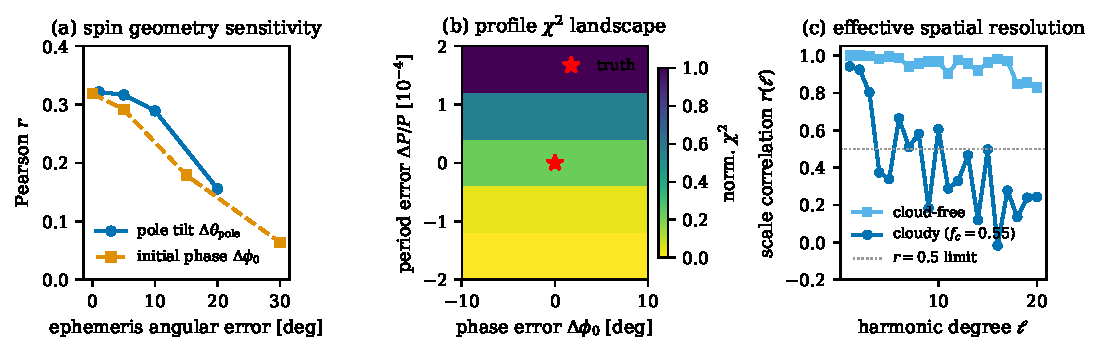
\includegraphics[width=0.95\textwidth]{figures/fig_robust.pdf}
\caption{Robustness of TDI at $f_c\simeq0.55$ (single seed). Left,
center: SSIM under mis-specified cloud decorrelation time and amplitude
(dotted lines: truth; dashed orange: white-noise GLS reference).
Right: sensitivity to rotation-period error---$10^{-4}$ is tolerable,
$10^{-3}$ is fatal, setting a precursor-knowledge requirement.}
\label{fig:robust}
\end{figure*}

\section{From Algorithm to Mission}
\label{sec:mission}

The lens is target-specific: the focal line extends anti-parallel to the
target direction, and a spacecraft cruising outward at
$\sim$150~km\,s$^{-1}$ has no meaningful capability to retarget
(a $1^\circ$ change of line-of-sight at 650~AU corresponds to an
11.3~AU lateral displacement; \citealt{tur26uhr,tur26prop}). Target
selection, trajectory, and onboard resources are therefore inseparable
from the imaging algorithm requirements derived above. This section
assembles them into a coherent mission picture.

\subsection{The five best targets and their focal-line placements}
\label{sec:targets}

Table~\ref{tab:targets} evaluates the five nearest {\it confirmed}
planets that current radial-velocity work places in or near their
stars' habitable zones, plus one solar-type alternative, as SGL imaging
targets. For each planet we list the adopted physical parameters
(discovery references in the table notes), and compute: the projected
image-cylinder diameter $D_{\rm img}$ at $z=650$~AU; the fiducial
photon rate $Q_{\rm exo}$ scaled from the 30~pc benchmark
($Q\propto S\,R_p\,z_0^{-1}$ at fixed $z$, $d$, $\lambda$;
\citealt{tt22mnras}) and the resulting per-dwell
$\mathrm{SNR_C}$(1800~s); the celestial placement of the focal line
(the antipode of the target's J2000 position, with its ecliptic
latitude); and the image-plane dynamics---the radius
$r_{\rm img}=a_p(z/z_0)$ and speed
$v_{\rm img}=v_{\rm orb}(z/z_0)$ of the circular track the planetary
image sweeps around the host star's focal line each planetary year,
together with the $\Delta v$ a spacecraft would expend to track the
image continuously for 90~days. Radii for these non-transiting planets
are estimated from $M\sin i$ via a rocky mass--radius relation
$R\propto M^{0.28}$ \citep{chenkipping17}; all photometric quantities
therefore carry the (unknown) $\sin i$ and albedo systematics, and
should be read as ranking metrics rather than forecasts.

\begin{table*}[t]
\centering
\caption{The five nearest confirmed potentially habitable planets (and
one solar-type alternative) as SGL imaging targets. Observing geometry
evaluated at $z=650$~AU, $d=1$~m, $\lambda=1\,\mu$m.}
\label{tab:targets}
\footnotesize
\setlength{\tabcolsep}{3.5pt}
\begin{tabular}{lccccccccccc}
\toprule
Planet & Host (SpT) & $z_0$ & $M\sin i$ & $R_p^{\,a}$ & $S$ & $P$ &
$D_{\rm img}$ & $\mathrm{SNR_C}$ & Focal direction$^{\,b}$ &
$\beta_{\rm ecl}$ & $\Delta v_{90}^{\,c}$ \\
 & & (pc) & ($M_\oplus$) & ($R_\oplus$) & ($S_\oplus$) & (d) & (km) &
(1800 s) & (J2000) & (deg) & (km s$^{-1}$) \\
\midrule
Proxima Cen b & Proxima (M5.5V) & 1.30 & 1.07 & 1.02 & 0.65 & 11.19 &
31.5 & 659 & $02^{\rm h}30^{\rm m}$, $+62^\circ41'$ & $+44.8$ & 5.8 \\
Ross 128 b & Ross 128 (M4V) & 3.38 & 1.35 & 1.09 & 1.38 & 9.87 &
12.9 & 576 & $23^{\rm h}48^{\rm m}$, $-00^\circ48'$ & $+0.5$ & 2.9 \\
GJ 1061 d & GJ 1061 (M5.5V) & 3.67 & 1.64 & 1.15 & 0.69 & 13.03 &
12.6 & 280 & $15^{\rm h}36^{\rm m}$, $+44^\circ31'$ & $+60.8$ & 1.7 \\
Teegarden c & Teegarden's Star (M7V) & 3.83 & 1.11 & 1.03 & 0.37 & 11.41 &
10.8 & 129 & $14^{\rm h}53^{\rm m}$, $-16^\circ53'$ & $-0.3$ & 1.7 \\
GJ 273 b & Luyten's Star (M3.5V) & 3.80 & 2.89 & 1.35 & 1.06 & 18.65 &
14.2 & 486 & $19^{\rm h}27^{\rm m}$, $-05^\circ14'$ & $+16.5$ & 1.3 \\
\midrule
$\tau$ Cet e$^{\,d}$ & $\tau$ Ceti (G8.5V) & 3.60 & 3.93 & 1.47 &
1.71 & 162.9 & 16.3 & 901 & $13^{\rm h}44^{\rm m}$, $+15^\circ56'$ &
$+24.8$ & 0.11 \\
\bottomrule
\end{tabular}

\vspace{1.5mm}
\parbox{0.94\textwidth}{\footnotesize
Image-plane sweep speeds $v_{\rm img}$ are 114, 51, 39, 35, 44, and
31~m\,s$^{-1}$ from top to bottom.
$^{a}$Estimated from $M\sin i$ via $R\propto M^{0.28}$
\citep{chenkipping17}; none of these planets transit.
$^{b}$Antipode of the host's J2000 position (arcminute precision); the
usable focal segment extends along this direction from $z\simeq548$~AU
outward, with 650--900~AU the practical operating range
\citep{tur26prop}. $\beta_{\rm ecl}$ is the ecliptic latitude of the
focal direction.
$^{c}$Propellant cost of continuously tracking the planetary image's
orbital sweep for 90 days, $\Delta v_{90}=a_{\rm img}\times90$~d;
picket-style sampling \citep{tt22dyn} reduces this dramatically.
$^{d}$Radial-velocity candidate, not confirmed; included as the nearest
potentially habitable planet of a solar-type star. Parameters:
\citet{anglada16,faria22} (Proxima b); \citet{bonfils18} (Ross 128 b);
\citet{dreizler20} (GJ 1061 d); \citet{zechmeister19,dreizler24}
(Teegarden c); \citet{astudillo17} (GJ 273 b); \citet{feng17}
($\tau$ Cet e). Instellations from the discovery papers.}
\end{table*}

\begin{figure*}[t]
\centering
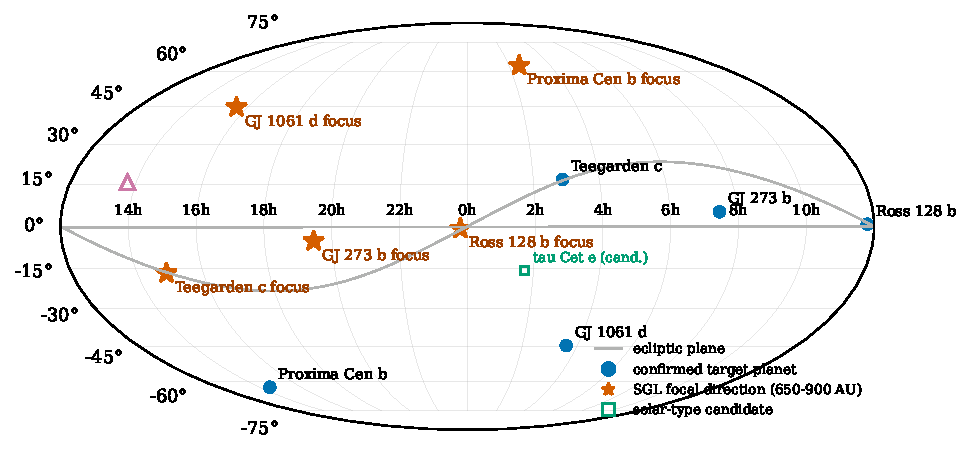
\includegraphics[width=0.9\textwidth]{figures/fig_targets.pdf}
\caption{Sky placement (equatorial Mollweide) of the five ranked targets
(blue circles) and their SGL focal directions (orange stars)---the
antipodal points toward which the spacecraft must cruise. The gray curve
is the ecliptic. Note that the Ross 128 and Teegarden focal lines lie
almost exactly in the ecliptic plane, while GJ 1061's focus is at
$+61^\circ$ ecliptic latitude, with consequences for launch geometry,
navigation-field stars, and zodiacal foregrounds.}
\label{fig:targets}
\end{figure*}

Several mission-shaping conclusions follow.

{\it 1. Proxima Centauri b} is the photometric and geometric optimum:
15 times the fiducial photon rate ($\mathrm{SNR_C}=659$ per 1800~s
dwell) and a 31.5~km image cylinder whose generous pixel spacing
essentially eliminates the deconvolution penalty (at $n=128$,
$0.891D/d\sqrt{N}>1$; even a $1024\times1024$ megapixel raster incurs
only a factor $\sim$0.03 penalty, so megapixel imaging of Proxima b is
photon-cheap: $\mathrm{SNR_R}\simeq18$ per 1800~s-per-pixel pass with
16 spacecraft in $\sim$3.7~yr of cumulative dwell). Its liabilities are
dynamical: the 11.2~d orbit sweeps the planetary image around the
stellar focal line at 114~m\,s$^{-1}$ (track radius $1.76\times10^4$~km),
so continuous tracking would cost 5.8~km\,s$^{-1}$ per 90~d---infeasible
for smallsats. Proxima b therefore forces the picket strategy analyzed
by \citet{tt22dyn}: spacecraft hold station near the stellar focal line
and sample the image during periodic sweeps, which our cadence result
actually favors (many short, phase-diverse encounters). The focal line
at $02^{\rm h}30^{\rm m}$, $+62^\circ41'$ (ecliptic latitude $+45^\circ$)
requires a high-inclination departure.

{\it 2. Ross 128 b} offers the best photon-dynamics compromise among
confirmed planets: $\mathrm{SNR_C}=576$, half Proxima's tracking burden,
a quiet M4 host \citep{bonfils18}, and a focal line lying {\it in} the
ecliptic ($\beta=+0.5^\circ$), the cheapest departure geometry.

{\it 3. GJ 1061 d} is the most temperate confirmed target
($S=0.69\,S_\oplus$) with moderate dynamics, but its focal line at
$+61^\circ$ ecliptic latitude is the most expensive to reach.

{\it 4. Teegarden c} orbits the least active host (M7V;
\citealt{dreizler24}), minimizing stellar-contamination systematics in
the Einstein ring, at the cost of the lowest photon rate
($\mathrm{SNR_C}=129$; still ample---corona-limited dwell budgets
scale as $\mathrm{SNR_C}^{-2}$ and remain subdominant to cloud noise).
Its focal line also lies in the ecliptic.

{\it 5. GJ 273 b (Luyten b)} is the most massive and thus most likely
to retain a substantial atmosphere; it combines high
$\mathrm{SNR_C}=486$ with the lowest tracking cost among the confirmed
five (1.3~km\,s$^{-1}$ per 90~d, thanks to its wider 18.65~d orbit).

{\it The solar-type alternative.} If $\tau$~Ceti~e is confirmed, it
becomes arguably the best imaging target of all: the highest photon
rate in the table ($\mathrm{SNR_C}=901$), and---because its habitable
zone lies at 0.54~AU rather than 0.05~AU---image-plane dynamics
{\it fifty times gentler} than Proxima b (0.11~km\,s$^{-1}$ per 90~d),
compatible with continuous tracking by modest electric propulsion. This
illustrates a general and previously underappreciated selection rule:
{\it M-dwarf habitable zones are photon-rich but dynamically expensive;
solar-type habitable zones are dynamically cheap.} Rotation periods
(Sec.~\ref{sec:robust}) are the second selection axis: tidally
synchronized M-dwarf planets ($P_{\rm rot}=P_{\rm orb}$, known to
$10^{-5}$ from RV ephemerides) automatically satisfy the $10^{-4}$
period requirement, converting a liability of M-dwarf targets into an
asset---though synchronization also fixes the illuminated hemisphere,
halving the mappable surface.

Since the mission is irrevocably single-target \citep{tur26uhr}, the
final selection must await precursor characterization (atmosphere
detection, rotation state, cloud statistics from disk-integrated
variability) by ELT-class and Habitable Worlds Observatory-era
facilities; the ranking above identifies where that precursor effort
buys the most mission risk reduction.

\subsection{Getting there: deep-perihelion sailcraft}
\label{sec:sail}

Reaching $z=650$~AU within a 20~yr program implies a mean radial speed
of 32.5~AU\,yr$^{-1}$ ($154$~km\,s$^{-1}$)---far beyond chemical or
gravity-assist propulsion, whose flight-heritage maximum is
3--4~AU\,yr$^{-1}$ \citep{tur26prop}. The schedule-credible path is
photonic: drop toward the Sun, deploy a large low-mass sail near
perihelion $r_p$, and exit hyperbolically with
\begin{equation}
v_\infty\simeq\sqrt{\frac{2\mu_\odot\beta}{r_p}},\qquad
\beta=\frac{p_0}{\sigma_{\rm tot}\,g_\odot(1\,{\rm AU})},
\end{equation}
where $\mu_\odot=GM_\odot$, $p_0=9.08~\mu$N\,m$^{-2}$, and
$\sigma_{\rm tot}$ is the
{\it total} system areal density including payload and---critically---
the non-solar power source \citep{tur26prop}. The quantitative
requirements are stringent: at $r_p=0.05$~AU (10.7~$R_\odot$),
$v_\infty\simeq105$~km\,s$^{-1}$ (30~yr class) requires
$\sigma_{\rm tot}\simeq4.9$~g\,m$^{-2}$, and
$v_\infty\simeq155$~km\,s$^{-1}$ (20~yr class) requires
$\sigma_{\rm tot}\simeq2.3$~g\,m$^{-2}$; a 100~kg sailcraft at
$\sigma_{\rm tot}=4.9$~g\,m$^{-2}$ implies a $2\times10^4$~m$^2$
($\sim$140~m square) sail. Thin-membrane equilibrium at $r_p=0.05$~AU
reaches $\sim$740~K (for absorptivity 0.05, emissivity 0.8), and a
representative 50~kg, $10^4$~m$^2$ point design achieving 21~AU\,yr$^{-1}$
from $r_p=0.025$~AU saw 950~K \citep{helvajian23}. Sail deployment at
10~m scale is flight-proven, but deep-perihelion material systems are at
low technology readiness; the 25--40~yr-class regime
($r_p\sim0.05$--0.1~AU, $\sigma_{\rm tot}$ of a few g\,m$^{-2}$) is the
realistic near-term envelope, with sub-20~yr access gated by a focused
materials-and-deployment qualification program \citep{tur26prop}.

The alternatives trade schedule for capability. Nuclear electric
propulsion with a 20~t stage, 800~kg payload, $I_{\rm sp}=9000$~s and
specific mass $\alpha_{\rm tot}=10$--20~kg\,kW$_e^{-1}$ reaches 650~AU
in 27--33~yr while delivering hundreds of kW$_e$ for operations; sub-20~yr
NEP requires either $\alpha_{\rm tot}\lesssim3$~kg\,kW$_e^{-1}$ or a
hybrid architecture in which an Oberth-maneuver injection stage
(e.g., nuclear-thermal, firing at $r_p\sim0.02$~AU) supplies
$v_0\simeq50$--70~km\,s$^{-1}$ before the NEP cruise
\citep{tur26prop}. For the swarm-heavy architectures our cadence law
favors (Sec.~\ref{sec:cadence}), the sail-first roadmap is the natural
match: each $\lesssim$100~kg ``pearl'' rides its own sail, launches are
staggered at 1--2~yr intervals so that later pearls carry improved
technology \citep{helvajian23}, and the large sail area is retained at
the focal region for reuse as a solar occulter \citep{tur26prop}.

\subsection{Power and communications at 500--1000 AU}
\label{sec:power}

Beyond $\sim$500~AU solar flux is $4\times10^5$--$8\times10^5$ times
weaker than at 1~AU: photovoltaics are useless and every watt must be
nuclear \citep{tur26prop}. The conventional option, the Multi-Mission
Radioisotope Thermoelectric Generator, supplies $\sim$110~W$_e$ at
$\lesssim$45~kg---a 20--50\% mass fraction for a 100--200~kg sailcraft
that directly inflates $\sigma_{\rm tot}$ and, through
$v_\infty\propto\sigma_{\rm tot}^{-1/2}$, the trip time; indeed a 1~kW$_e$
system at 100~kg\,kW$_e^{-1}$ adds sail area equivalent to an 80~m-radius
disk just to carry its own power supply \citep{tur26prop}. The
architecture developed for exactly this problem is the Atomic Planar
Power for Lightweight Exploration (APPLE) concept: modular
$10\times10\times1.7$~cm tiles integrating $^{238}$Pu heat sources with
thermoelectric converters and radiation-hard solid-state batteries,
each tile delivering $\ge$1.2~W$_e$ continuously plus 5~Wh of storage
for $\ge$15~yr, with decay heat keeping the battery warm without
electrical heaters \citep{apple22,niac20}. Tiled power scales from watts
to hundreds of watts at areal mass compatible with sailcraft, and the
battery buffers the peak loads of our observing concept---short
high-duty-cycle dwells, image-plane maneuvering, and burst downlink.

The data volume demanded by time-domain imaging is modest. Each sample
is a time-tagged photometric integral ($\lesssim$32~bytes); the fiducial
campaign produces $6.6\times10^4$ samples ($\sim$2~MB), and even a
megapixel, 64-visit Proxima campaign totals $\sim$2~GB of raw
photometry. Optical-communication architectures studied for the
string-of-pearls concept---inter-pearl laser relays hopping down the
line of spacecraft, with the innermost ``caboose'' pearl closing the
link to Earth---project tens to hundreds of kb\,s$^{-1}$ from
500--800~AU \citep{helvajian23}, i.e., days per full raster: downlink
is not a driver. The binding resource conclusions are instead (i)
per-pearl power of order 10$^2$~W$_e$ (tiled RPS), (ii) transverse
image-plane mobility budgets of 0.1--5.8~km\,s$^{-1}$ per 90~d depending
on target (Table~\ref{tab:targets}), and (iii) the swarm multiplicity
itself, which our cadence law sets at $\mathcal{O}(10^2)$ registered
visits per pixel for Earth-like cloud cover---achievable as
$16\ {\rm craft}\times{\rm years}$ or $10^2\ {\rm craft}\times90$~d.

\section{Discussion and Limitations}
\label{sec:discussion}

Our simulations are deliberately transparent rather than exhaustive, and
several simplifications bound the claims. (i) We use the monopole,
aperture-averaged SGL response; the solar quadrupole breaks the PSF into
caustics that increase the deconvolution burden \citep{tt21quad}, and
extending TDI with a $J_2$-dependent kernel library is the most
important optical upgrade. (ii) The corona enters as Gaussian shot noise
with its mean assumed subtracted; structured coronal residuals and
calibration drifts---shown by \citet{tur26bench} to demand sub-ppm
effective flat-fielding---are not modeled. (iii) The cloud field is a
single-layer stochastic opacity screen without radiative transfer,
phase-angle dependence, or climate structure; it is calibrated,
however, so that the estimator never receives information unavailable
to a real mission, and the robustness scans show factor-of-few
climatology errors are benign. (iv) The geometry is a single equatorial,
zero-obliquity case; oblique and pole-on geometries redistribute (but do
not eliminate) the rotational information TDI exploits. (v) Navigation
is perfect: pointing jitter and image-plane ephemeris error enter as an
additional convolution and their coupling to the $10^{-4}$
rotation-period requirement deserves a dedicated study. (vi) Truth maps
live on a finer grid than the reconstruction, dwell-smear is present in
data but not operator, and tuning constants were frozen on held-out
seeds---standard inverse-crime mitigations, though only flight-like
simulation chains \citep{tur26bench} can retire the concern fully.
(vii) Our per-pixel temporal covariance is the simplest member of the
covariance-aware family; the measured gap to the cloud-free ceiling
(factor $\sim$3 in $r$ at Earth-like cover) quantifies the prize for
full spatio-temporal cloud modeling, e.g., joint estimation of a
low-order cloud state per epoch or GCM-informed priors, in the spirit
of \citet{cov26}.

These caveats do not touch the two structural results---that
rotation-aware joint inversion removes the temporal-aliasing penalty,
and that cloud noise, being temporally correlated nuisance variance
rather than photon noise, is purchasable with revisits rather than
photons. Both follow from the linearity of the measurement and the
separation of timescales ($P_{\rm rot}\ll\tau_c\ll T_{\rm camp}$), not
from details of our cloud model.

\section{Conclusions}
\label{sec:conclusions}

We built a validated, open, end-to-end simulator of exoplanet imaging
with the solar gravitational lens---reproducing the published kernel,
photon-rate, and deconvolution-penalty benchmarks---and used it to
attack the time-domain inverse problem that the current literature
identifies as the concept's leading unsolved challenge. Our conclusions:

1. Time-domain inversion (regularized GLS on time-tagged samples with
the rotation/illumination ephemeris in the forward operator) recovers a
rotating, cloud-free planet with $r=0.99$, SSIM $=0.92$---removing the
$\mathrm{SNR}\lesssim2$ barrier of earlier dynamic reconstructions and
demonstrating that planetary rotation, per se, costs SGL imaging almost
nothing.

2. Clouds dominate the noise budget, exceeding coronal shot noise
per sample by factors of 14--23 for covers of 22--72\%. At
single-campaign budgets, fidelity collapses to $r\simeq0.26$--0.33 at
Earth-like cover for every estimator tested, quantitatively confirming
published caution---but the gross land--ocean dichotomy survives.

3. Cloud noise is correlated, and that is exploitable. A globally
correlated mode (injected by the $1/\rho$ kernel wings) is removable by
per-slot deflation; the temporal correlation defines an
observing-cadence law: at fixed photons and wall-clock, 64 short
revisits outperform 4 long dwells by a factor $\sim$4 in $r$. Cadence,
not collecting area, is the control knob for cloudy targets, and it
directly sizes multi-spacecraft swarms: $\mathcal{O}(10^2)$ registered
visits per pixel for high-fidelity mapping under Earth-like clouds.

4. The method needs the rotation period to $\sim10^{-4}$ and only
order-of-magnitude cloud climatology---a clean, achievable precursor
requirement set.

5. Among the five nearest confirmed potentially habitable planets,
Proxima~b is photon-optimal but dynamically expensive
(image sweeps at 114~m\,s$^{-1}$; 5.8~km\,s$^{-1}$ per 90~d of
continuous tracking), Ross 128~b offers the best compromise with an
in-ecliptic focal line, and GJ 273~b minimizes tracking cost; a
confirmed $\tau$~Ceti~e would dominate the ranking outright. Focal-line
placements, photon rates, and tracking budgets for all targets are
tabulated for mission design.

6. The transportation and resource stack is consistent with the
current architecture literature: deep-perihelion sailcraft
($\sigma_{\rm tot}\simeq2.3$--4.9~g\,m$^{-2}$ at $r_p=0.05$~AU for
155--105~km\,s$^{-1}$), tiled radioisotope power ($\ge$1.2~W$_e$ per
$10\times10\times1.7$~cm APPLE tile), and optical relay downlink at
tens of kb\,s$^{-1}$---with the swarm multiplicity demanded by our
cadence law emerging as the single strongest architectural driver.

The time-domain problem, in short, is not a veto but a design driver:
it converts ``can the SGL image a living, breathing planet?'' into
specific, testable requirements on cadence, swarm size, precursor
ephemerides, and covariance modeling. All code, seeds, and data needed
to reproduce every number in this paper accompany the manuscript.

\acknowledgments
This work used only publicly available literature and open-source
software (NumPy, SciPy, Matplotlib, scikit-image). The author thanks
the maintainers of the arXiv and of the SGL literature for making this
analysis possible, and declares no external funding.

\appendix

\section{Solver implementation}
\label{app:solver}
The normal equations of Eq.~(\ref{eq:tdi}) are assembled per
image-plane pixel: for pixel $p$ with visit set $\mathcal{V}_p$
($|\mathcal{V}_p|=M_p$), the local covariance
$\mathsf{C}_p=\sigma_{\rm cl}^2\,\mathsf{T}_p+
\mathrm{diag}(\sigma_k^2)$,
$(\mathsf{T}_p)_{ij}=e^{-|t_i-t_j|/\tau_c}$, is Cholesky-factored
($M_p\times M_p$) and applied to the corresponding rows of
$\mathsf{F}$ and entries of $\mathbf{y}$; whitened blocks are
accumulated into
$\mathsf{A}=\mathsf{F}^{\sf T}\mathsf{C}^{-1}\mathsf{F}$ and
$\mathbf{b}=\mathsf{F}^{\sf T}\mathsf{C}^{-1}\mathbf{y}$ in single
precision and solved in double precision. Slot deflation subtracts from
each sample (and operator row) the mean over the $N_{\rm sc}$
simultaneous samples of its dwell slot, and rescales the white-noise
term by $\sqrt{1-1/N_{\rm sc}}$; it is an orthogonal projection, so the
deflated GLS remains unbiased for $\mathbf{s}$ up to the removed global
mode, which is restored by the climatological de-bias. The
regularization weight is dimensionless:
$\lambda_{\rm eff}=\lambda\,\mathrm{tr}(\mathsf{A})/
\mathrm{tr}(\mathsf{L}^{\sf T}\mathsf{L})$ with $\lambda=3\times10^{-3}$
for all results. Building the $65{,}536\times2592$ operator takes
$\sim$3~s and each solve $\sim$10~s (two CPU cores).

\section{Reproducibility}
\label{app:repro}
The archive accompanying this paper contains \texttt{code/sglsim.py}
(physics, scene, campaign, estimators; $\sim$600 lines),
\texttt{code/run\_experiments.py} (checkpointed experiment driver),
\texttt{code/targets.py} (Table~\ref{tab:targets} and
Fig.~\ref{fig:targets}), and \texttt{code/make\_figures.py}. All random
processes are seeded; the seeds used here are 7 (truth map), 2026
(campaign), 11--13 (noise/cloud realizations), 99/199 (held-out
calibration), and 999 (climatology probes). Every number quoted in the
text and tables regenerates from
\texttt{run\_experiments.py} in $\sim$40 core-minutes.

\begin{thebibliography}{}

\bibitem[Anglada-Escud\'e et al.(2016)]{anglada16}
Anglada-Escud\'e, G., Amado, P.~J., Barnes, J., et al.\ 2016, Nature,
536, 437

\bibitem[Astudillo-Defru et al.(2017)]{astudillo17}
Astudillo-Defru, N., Forveille, T., Bonfils, X., et al.\ 2017, A\&A,
602, A88

\bibitem[Baumbach(1937)]{baumbach37}
Baumbach, S.\ 1937, Astron.\ Nachr., 263, 121

\bibitem[Bonfils et al.(2018)]{bonfils18}
Bonfils, X., Astudillo-Defru, N., D\'iaz, R., et al.\ 2018, A\&A, 613,
A25

\bibitem[Chen \& Kipping(2017)]{chenkipping17}
Chen, J., \& Kipping, D.\ 2017, ApJ, 834, 17

\bibitem[Dreizler et al.(2020)]{dreizler20}
Dreizler, S., Jeffers, S.~V., Rodr\'iguez, E., et al.\ 2020, MNRAS,
493, 536

\bibitem[Dreizler et al.(2024)]{dreizler24}
Dreizler, S., Luque, R., Ribas, I., et al.\ 2024, A\&A, 684, A117
(arXiv:2402.00923)

\bibitem[Eshleman(1979)]{eshleman79}
Eshleman, V.~R.\ 1979, Science, 205, 1133

\bibitem[Faria et al.(2022)]{faria22}
Faria, J.~P., Su\'arez Mascare\~no, A., Figueira, P., et al.\ 2022,
A\&A, 658, A115

\bibitem[Feng et al.(2017)]{feng17}
Feng, F., Tuomi, M., Jones, H.~R.~A., et al.\ 2017, AJ, 154, 135

\bibitem[Friedman et al.(2024)]{friedman24}
Friedman, L.~D., Garber, D., Turyshev, S.~G., et al.\ 2024, Exp.\
Astron., 57, 1 (arXiv:2107.11473)

\bibitem[Helvajian et al.(2023)]{helvajian23}
Helvajian, H., Rosenthal, A., Poklemba, J., et al.\ 2023, J.\ Spacecr.\
Rockets, 60, 829 (arXiv:2207.03005)

\bibitem[Madurowicz \& Macintosh(2022)]{mm22}
Madurowicz, A., \& Macintosh, B.\ 2022, ApJ, 930, 19 (arXiv:2204.13811)

\bibitem[NASA/Aerospace Corp.(2022)]{apple22}
Aerospace Corporation \& NASA NIAC 2022, Atomic Planar Power for
Lightweight Exploration (APPLE), NIAC Phase II study,
\url{https://www.nasa.gov/directorates/spacetech/niac/2022/Atomic_Planar_Power}

\bibitem[Perlin(1985)]{perlin85}
Perlin, K.\ 1985, ACM SIGGRAPH Comput.\ Graph., 19, 287

\bibitem[Richardson(1972)]{richardson72}
Richardson, W.~H.\ 1972, J.\ Opt.\ Soc.\ Am., 62, 55

\bibitem[Teinturier et al.(2022)]{teinturier22}
Teinturier, L., Vieira, N., Jacquet, E., et al.\ 2022, MNRAS, 511, 440

\bibitem[Toth(2024)]{toth24}
Toth, V.~T.\ 2024, MNRAS, 527, 1141

\bibitem[Toth(2025)]{toth25clouds}
Toth, V.~T.\ 2025, Res.\ Astron.\ Astrophys., in press
(arXiv:2504.18630)

\bibitem[Toth \& Turyshev(2021)]{toth21}
Toth, V.~T., \& Turyshev, S.~G.\ 2021, Phys.\ Rev.\ D, 103, 124038

\bibitem[Toth \& Turyshev(2023)]{toth23}
Toth, V.~T., \& Turyshev, S.~G.\ 2023, MNRAS, 525, 5846

\bibitem[Turyshev(2026a)]{tur26direct}
Turyshev, S.~G.\ 2026, Phys.\ Rev.\ D, 113, 023034 (arXiv:2506.20236)

\bibitem[Turyshev(2026b)]{tur26bench}
Turyshev, S.~G.\ 2026, arXiv:2606.14899

\bibitem[Turyshev(2026c)]{tur26uhr}
Turyshev, S.~G.\ 2026, arXiv:2606.18300

\bibitem[Turyshev(2026d)]{tur26prop}
Turyshev, S.~G.\ 2026, arXiv:2602.04198

\bibitem[Turyshev(2026e)]{cov26}
Turyshev, S.~G.\ 2026, arXiv:2606.29138

\bibitem[Turyshev \& Toth(2017)]{tt17}
Turyshev, S.~G., \& Toth, V.~T.\ 2017, Phys.\ Rev.\ D, 96, 024008

\bibitem[Turyshev \& Toth(2019)]{tt19}
Turyshev, S.~G., \& Toth, V.~T.\ 2019, Phys.\ Rev.\ D, 99, 024044

\bibitem[Turyshev \& Toth(2020)]{tt20psf}
Turyshev, S.~G., \& Toth, V.~T.\ 2020, Phys.\ Rev.\ D, 102, 024038

\bibitem[Turyshev \& Toth(2021)]{tt21quad}
Turyshev, S.~G., \& Toth, V.~T.\ 2021, Phys.\ Rev.\ D, 103, 064076

\bibitem[Turyshev \& Toth(2022a)]{tt22mnras}
Turyshev, S.~G., \& Toth, V.~T.\ 2022a, MNRAS, 515, 6122

\bibitem[Turyshev \& Toth(2022b)]{tt22dyn}
Turyshev, S.~G., \& Toth, V.~T.\ 2022b, Phys.\ Rev.\ D, 105, 044012

\bibitem[Turyshev \& Toth(2022c)]{tt22spec}
Turyshev, S.~G., \& Toth, V.~T.\ 2022c, Phys.\ Rev.\ D, 106, 044059

\bibitem[Turyshev et al.(2020)]{niac20}
Turyshev, S.~G., Shao, M., Toth, V.~T., et al.\ 2020, Direct Multipixel
Imaging and Spectroscopy of an Exoplanet with a Solar Gravity Lens
Mission, NASA NIAC Phase II Final Report (arXiv:2002.11871)

\bibitem[Wang et al.(2004)]{wang04}
Wang, Z., Bovik, A.~C., Sheikh, H.~R., \& Simoncelli, E.~P.\ 2004, IEEE
Trans.\ Image Process., 13, 600

\bibitem[Zechmeister et al.(2019)]{zechmeister19}
Zechmeister, M., Dreizler, S., Ribas, I., et al.\ 2019, A\&A, 627, A49

\end{thebibliography}

\end{document}
